
\section{The Electric Field of the Atomic Nucleus}

Name \rule{2.0in}{0.1pt}\hfill{}Section \rule{1.0in}{0.1pt}\hfill{}Date
\rule{1.0in}{0.1pt}

\textbf{Introduction}

In this exercise you will make a theoretical investigation of the
electric field associated with the atomic nucleus. Our current understanding
of the nucleus is the product of scattering experiments where a projectile
(e.g. an electron, photon, or even another nucleus) is given an initial
kinetic energy and collides with a target nucleus (see figure below). 

\vspace{0.3cm}
{\centering \resizebox*{0.45\textwidth}{!}{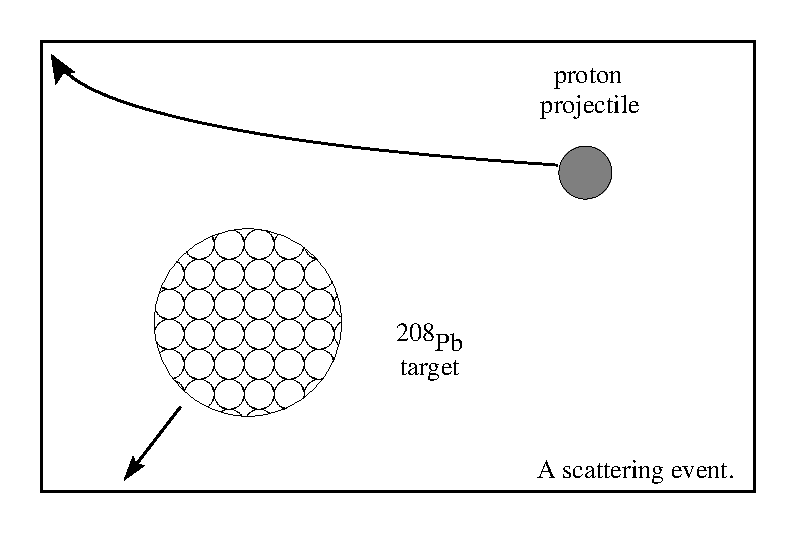
\includegraphics{electric_field_atomic_nucleus/electric_field_atomic_nuleus_fig_1.eps}} \par}
\vspace{0.3cm}

The final energies and velocities of the products of the reaction
are then measured and the nature of the interaction is inferred. There
are several important features of the nucleus that can be learned
from these experiments:

\begin{enumerate}
\item The nucleus is small, about 100,000 times smaller than the atom itself.
\item Most of the matter and all of the positive charge is located in this
tiny object.
\item There exists a force, called the strong force, that is attractive,
acts only within the volume of the nucleus, and is powerful enough
to overcome the repulsion between the positive charges concentrated
in the nucleus. 
\end{enumerate}
Below you will calculate the electric field of the \( ^{208} \)Pb
nucleus and the force between an incident proton and \( ^{208} \)Pb.
You will also calculate the work necessary to penetrate the nucleus.

\textbf{Activity 1: The Electric Field of \( ^{208} \)Pb}

(a) From scattering experiments like those described above one finds
that the positive charge of \( ^{208} \)Pb is uniformly distributed
throughout the volume of the nucleus, which can be treated as a sphere
of radius 7.11 x 10\( ^{-15} \) m or in units common to nuclear physics,
7.11 fm, where {}``fm'' is known as a fermi. Calculate the total
charge, Q, of the \( ^{208} \)Pb nucleus.
\vspace{30mm}

(b) Calculate the volume charge density, \( \rho  \), of the \( ^{208} \)Pb
nucleus.
\vspace{30mm}

(c) Starting with Gauss' Law, generate an expression for the electric
field, \textbf{E}, outside of the \( ^{208} \)Pb nucleus as a function
of $r$, the distance from the center of the sphere. Show and explain
each step of the calculation.
\vspace{2in}

(d) Use Gauss' Law to find an expression for \textbf{E} inside the
nucleus as a function of $r$. Show and explain each step of the calculation.
\vspace{2in}

(e) Construct a data table with the column headings $r$ (fm), $E$ (N/C),
and $F$ (N) in the space below. Then use the expressions you derived
above to calculate the electric field for at least ten radial positions
between 0 and 20 fm and enter the results in the table. Include 7.11
fm as one of your radial positions.
\vspace{3in}

\textbf{Activity 2: The force on a Proton}

(a) Consider a head-on collision between a proton and the \( ^{208} \)Pb
nucleus. Generate an expression for the force on the proton as a function
of $r$ outside the lead nucleus.
\vspace{20mm}

\vspace{1in}
(b) Calculate an expression for the force on the proton as a function
of $r$ inside the lead nucleus.
\vspace{30mm}

(c) Use these expressions to calculate the force at the same radial
positions where you calculated $E$ and enter the results in the table.

(d) Graph $F$ ($y$ axis) vs. $r$ and attach a copy to this unit.
\vspace{10mm}

\textbf{Activity 3: The Work Done by the Field}

(a) Recall that the work done by a force is \( W=\int ^{r_{f}}_{r_{i}}\overrightarrow{F}\cdot d\overrightarrow{s} \)
where r\( _{i} \) and r\( _{f} \) are the initial and final positions
of the object in motion. Treat the \( ^{208} \)Pb nucleus as a fixed
target and calculate the work done by the Coulomb force on the proton
if the proton approaches from infinity and reaches the surface of
the lead nucleus. Show all work.
\vspace{40mm}

(b) We know that the nuclear force binds particles like neutrons and
protons together once they enter the nucleus. From the graph of the
force as a function of position, what is the minimum strength of the
nuclear force in \( ^{208} \)Pb that will bind the proton in the
nucleus? Clearly state your reasoning.
\vspace{15mm}

(c) Consider a proton that has just enough initial kinetic energy
to move from infinitely far away and just reach the surface of the
lead nucleus. How is the initial kinetic energy related to the work
done by the field?
\vspace{15mm}

(d) How would the trajectory of the proton be affected if the kinetic
energy is less?
\vspace{15mm}

(e) How would the trajectory of the proton be affected if the kinetic
energy is greater?
\vspace{15mm}

(f) What minimum kinetic energy is needed for a proton to probe the
nucleus? Explain.\vspace{20mm}

